% -*- root: Dissertation.tex -*-
\documentclass[Dissertation.tex]{subfiles}
\graphicspath{{../Figures/}}
\begin{document}
\chapter{Entropy Norms for Compressible Navier-Stokes}
\label{sec:EntropyNorm}
\section{Motivation}

From the previous appendix, let $W$, $U$, and $V$ denote the set of primitive, conservation, and
entropy variables respectively.
% Define entropy function
It is well known that the entropy function
\[
H=-\rho\log(p\rho^{-\gamma})\,.
\]
provides a natural residual for the system of equations.
The Hessian of $H$ is known as the symmetrizer of the Navier-Stokes system
$A_0=H_{,UU}$, and $(U,A_0U)$ provides a physically consistent, entropy based metric.
By definition of the entropy variables (see \cite{HughesEntropyVariables}) $V_{,U}=H_{,UU}$, where
\[
V_{,U}(U)=\arrthree
{\frac{4\gamma\rho^2E^2-4\gamma\rho E\bfm\cdot\bfm+(1+\gamma)(\bfm\cdot\bfm)^2}{\rho(\bfm\cdot\bfm-2\rho E)^2}}
{-\frac{2\bfm\bfm\cdot\bfm}{\LRp{\bfm\cdot\bfm-2\rho E}^2}}
{-\frac{4\rho(\rho E-\bfm\cdot\bfm)}{\LRp{\bfm\cdot\bfm-2\rho E}^2}}
{}
{\frac{2\rho(2\rho E+\bfm\cdot\bfm)}{\LRp{\bfm\cdot\bfm-2\rho E}^2}}
{-\frac{4\rho^2\bfm}{\LRp{\bfm\cdot\bfm-2\rho E}^2}}
{Symm.}
{}
{\frac{4\rho^3}{\LRp{\bfm\cdot\bfm-2\rho E}^2}}\,.
\]

Since our previous comparison of Navier-Stokes formulations showed no strong reason to 
prefer anything over primitive variables, we will choose to work with primitive variables 
in this appendix. 
As such, we need to perform a change of variables to find the symmetrizer for the set of primitive variables:
% Consider a change of variables to primitive variables: 
$U=U_{,W}W$.
Our entropy metric is then
\[
\LRp{U_{,W} W,V_{,U}U_{,W} W}=\LRp{ W,U_{,W}^TV_{,U}U_{,W} W}
\]
Then
\[
U_{,W}=\arrthree{1}{0}{0}{\bfu}{\rho}{0}{C_vT+\frac{1}{2}\bfu\cdot\bfu}{\rho\bfu}{C_v\rho}
\]
where $V_{,U}$ in primitive variables is
\[
V_{,U}(W)=\arrthree
{\frac{\gamma}{\rho}+\frac{(\bfu\cdot\bfu)^2}{4\rho C_v^2 T^2}}
{-\frac{\frac{1}{2}\bfu\cdot\bfu\bfu}{\rho C_v^2 T^2}}
{-\frac{(C_v T-\frac{1}{2}\bfu\cdot\bfu)}{\rho C_v^2 T^2}}
{}
{\frac{C_v T+\bfu\cdot\bfu}{\rho C_v^2 T^2}}
{-\frac{\bfu}{\rho C_v^2 T^2}}
{Symm.}
{}
{\frac{1}{\rho C_v^2 T^2}}
\]
and
\[
A_0(W)=U_{,W}^TV_{,U}U_{,W}=\arrthree
{\frac{\gamma-1}{\rho}}
{0}
{0}
{0}
{\frac{\rho}{C_v T}}
{0}
{0}
{0}
{\frac{\rho}{T^2}}\,.
\]
As a check, $(W,A_0(W)W)$ has consistent units of density.
% Let $A_0^p=U_{,W}^TV_{,U}U_{,W}$ denote the symmetrizer for primitive variables.

\section{Entropy Scaled Test Norms}
% Recall the argument leading to the necessary condition for a robust norm \eqref{eq:necessaryCondition}
We repeat the argument to develop the necessary condition for a robust norm, but where we replace the bound
on $\norm{u}$ with $\norm{A_0^\frac{1}{2}u}$.
Let $u$ represent all volume variables, $\hat u$ all interface variables, and $v$ all test variables.
We can write our ultra-weak formulation as
\[
b\LRp{\LRp{u,\hat u},v} = \LRp{u,A^* v}_{L^2} + \LRa{\uh, \jump{v}}_{\Gh}
\]
where $A^*$ represents the adjoint.
For conforming $v^*$ satisfying $A^* v^* = A_0u$
\begin{align*}
&\norm{A_0^\frac{1}{2}u}^2
=\frac{b(u,v^*)}{\norm{v^*}_V} \norm{v^*}_V\\
&\quad\leq\sup_{v^*\neq0}\frac{|b(u,v^*)|}{\norm{v^*}}\norm{v^*}
=\norm{u}_E \norm{v^*}_V\,.
\end{align*}
This defines a necessary condition for robustness, namely that
\begin{align}
\label{eq:entropyNecessaryCondition}
\norm{v^*}_V\lesssim\norm{A_0^\frac{1}{2}u}_{L^2}\,.
\end{align}
If this condition is satisfied, then we get our final result:
\begin{align*}
\norm{A_0^\frac{1}{2}u}_{L^2}\lesssim\norm{u}_E\,.
\end{align*}

We begin by loading our compressible Navier-Stokes adjoint equations with $A_0W$:
\begin{align*}
\frac{1}{\mu}M^*(\Psi)+K^*(\Grad V)&=0
\\
-\vecttwo{F^*}{C^*}(\Gradxt V)+G^*(\Grad\Psi)&=A_0W\,.
\end{align*}
Without proof, we suggest the existence of analogous lemmas \ref{lem:l2} and \ref{lem:convective}  
for this case, namely that there exist bounds
\begin{equation}
\norm{A_0^{-\frac{1}{2}}V}^2+\mu\norm{A_0^{-\frac{1}{2}}\Grad V}^2\leq\norm{A_0^\frac{1}{2}}^2
\end{equation}
\begin{equation}
\norm{A_0^{-\frac{1}{2}}\vecttwo{F^*}{C^*}(\Gradxt V)}\lesssim\norm{A_0^\frac{1}{2}}\,.
\end{equation}
These would hypothetically be derived by substituting the first adjoint equation into 
the second then multiplying both sides by
\[
A_0^{-\frac{1}{2}}e^tV
\]
and
\[
-A_0^{-\frac{1}{2}}\vecttwo{F^*}{C^*}(\Gradxt V)\,,
\]
respectively for each desired bound, then integrating over $Q$ and following similar manipulations as were done in said lemmas.
Assuming the existence of said bounds, the analogous entropy scaled robust and coupled robust norms
for compressible Navier-Stokes would be
\begin{align*}
\norm{\LRp{V,\Psi}}_{V,K}^2 &\coloneqq
\norm{A_0^{-\frac{1}{2}}(F^*+C^*)}_K^2
+ \mu\norm{A_0^{-\frac{1}{2}}K^*}_K^2
+ \min\LRp{\frac{\mu}{h^2},1}\norm{A_0^{-\frac{1}{2}}V}^2_K
\\\nonumber&\quad
+ \norm{A_0^{-\frac{1}{2}}G^*}_K^2
+ \min\LRp{\frac{1}{\mu},\frac{1}{h^2}}\norm{A_0^{-\frac{1}{2}}M^*}_K^2\,,
\end{align*}
and
\begin{align*}
\norm{\LRp{V,\Psi}}_{V,K}^2 &\coloneqq
\norm{A_0^{-\frac{1}{2}}(F^*+C^*)}_K^2
+ \mu\norm{A_0^{-\frac{1}{2}}K^*}_K^2
+ \min\LRp{\frac{\mu}{h^2},1}\norm{A_0^{-\frac{1}{2}}V}^2_K
\\\nonumber&\quad
+ \norm{A_0^{-\frac{1}{2}}(G^*-F^*-C^*)}_K^2
+ \min\LRp{\frac{1}{\mu},\frac{1}{h^2}}\norm{A_0^{-\frac{1}{2}}M^*}_K^2\,.
\end{align*}
Note that in practice, $\rho$ and $T$ may get very close to 0 which can make the
Gram matrix for the test space inner product singular. In order to avoid this,
we bound the $\rho$ and $T$ terms in $A_0$ such that they are always greater than or equal
to 0.01.

We attempted two comparisons of the robust norm and the entropy scaled robust norm. 
The results for the Sod shock tube are very comparable, but the Newton iterations
failed to converge on the Noh problem.
We chalk this up as an interesting mathematical investigation, but a little disappointing numerically.
Besides, the equations have already been nondimensionalized, so it seems slightly superfluous
to additionally use the concept of entropy to develop consistent test norms.

\begin{figure}[ht]
\centering
\begin{subfigure}[t]{0.9\textwidth}
\centering
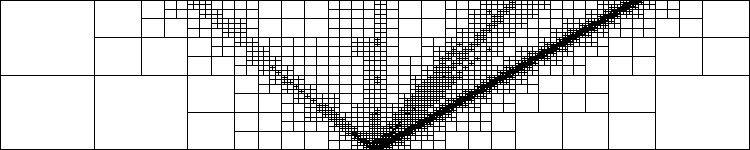
\includegraphics[width=\textwidth]{Dissertation/Sod/Robust-meshonly12.png}
\caption{Final mesh with robust norm}
\end{subfigure}
\begin{subfigure}[t]{0.9\textwidth}
\centering
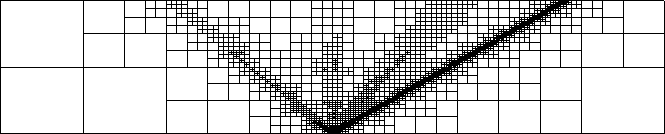
\includegraphics[width=\textwidth]{Dissertation/Sod/EntropyRobust-meshonly12.png}
\caption{Final mesh with entropy scaled robust norm}
\end{subfigure}
\begin{subfigure}[t]{0.9\textwidth}
\centering
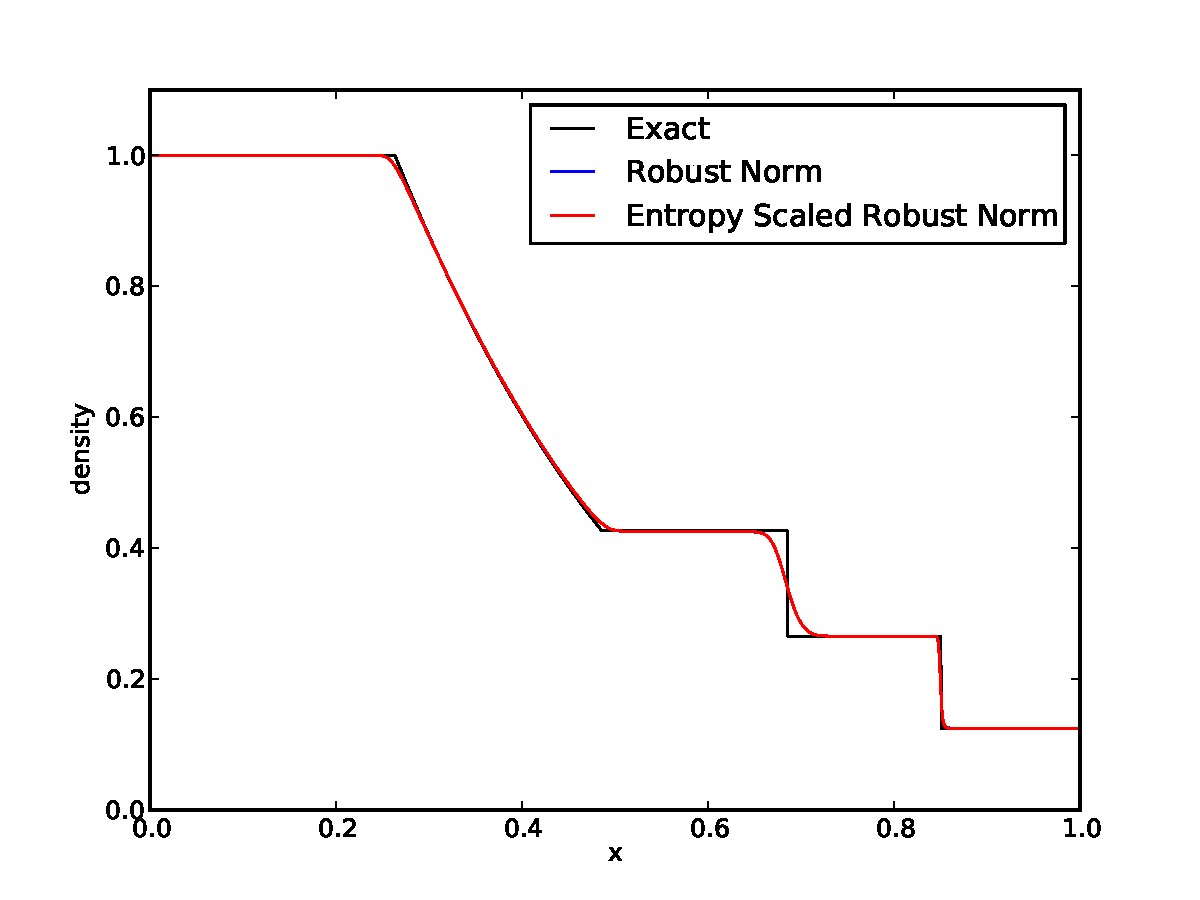
\includegraphics[width=\textwidth]{Dissertation/Sod/EntropyNormComparison-den.pdf}
\caption{Density at final time}
\end{subfigure}
\caption{Sod solution after 12 refinements}
\label{fig:SodEntropyComparison}
\end{figure}

% \begin{figure}[ht]
% \centering
% \begin{subfigure}[t]{0.45\textwidth}
% \centering
% 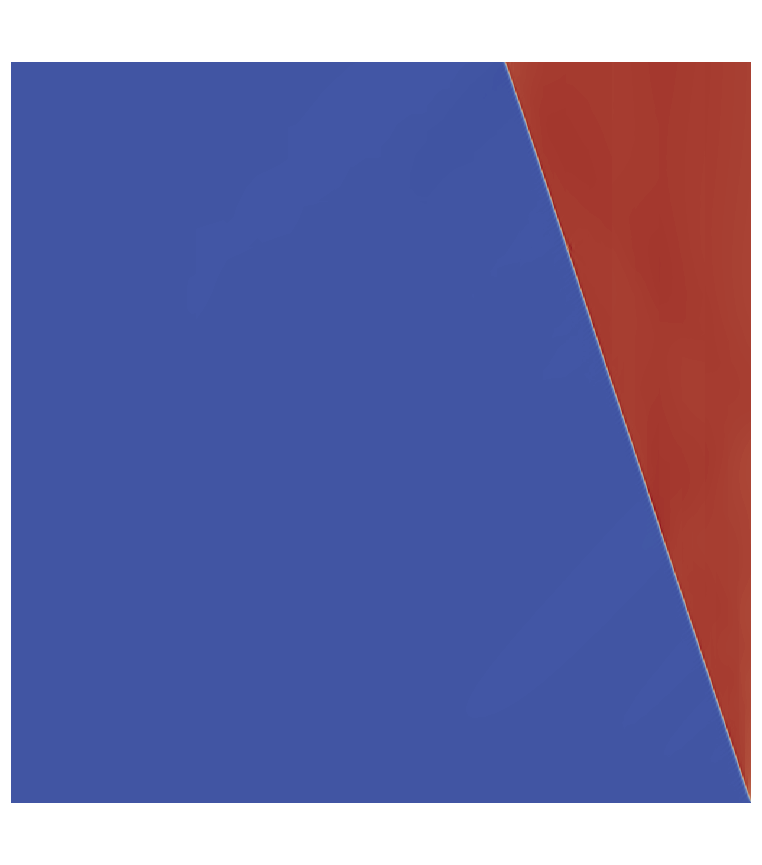
\includegraphics[width=\textwidth]{Dissertation/Noh/Robust-den10.png}
% \caption{Final density with robust norm}
% \end{subfigure}
% \begin{subfigure}[t]{0.45\textwidth}
% \centering
% 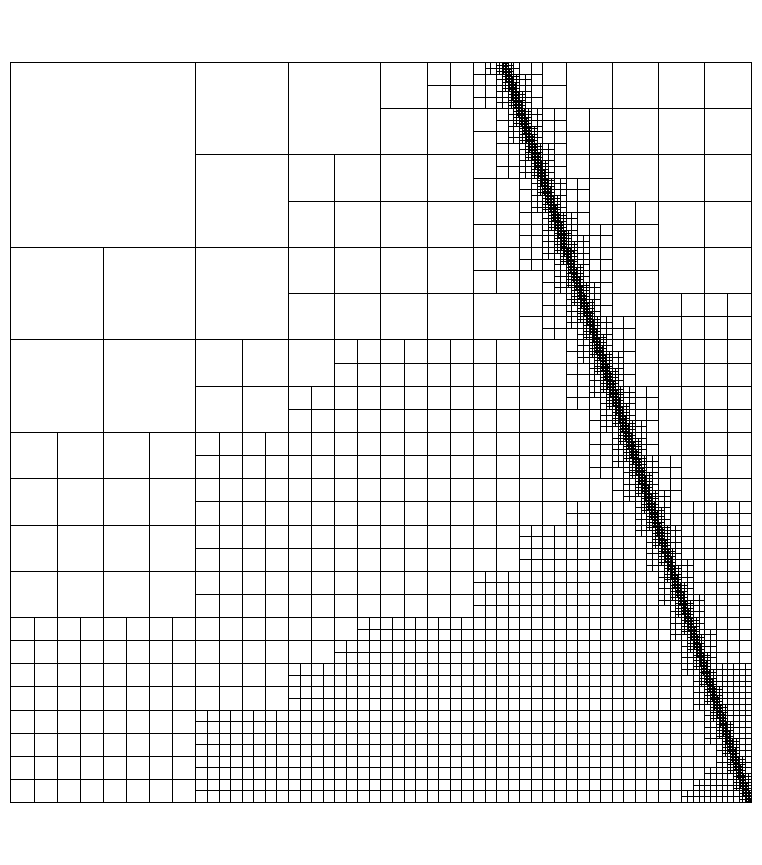
\includegraphics[width=\textwidth]{Dissertation/Noh/Robust-meshonly10.png}
% \caption{Final mesh with robust norm}
% \end{subfigure}
% \begin{subfigure}[t]{0.45\textwidth}
% \centering
% 
\includegraphics[width=\textwidth]{Dissertation/Noh/EntropyRobust-den10.png}
% \caption{Final density with entropy scaled robust norm}
% \end{subfigure}
% \begin{subfigure}[t]{0.45\textwidth}
% \centering
% 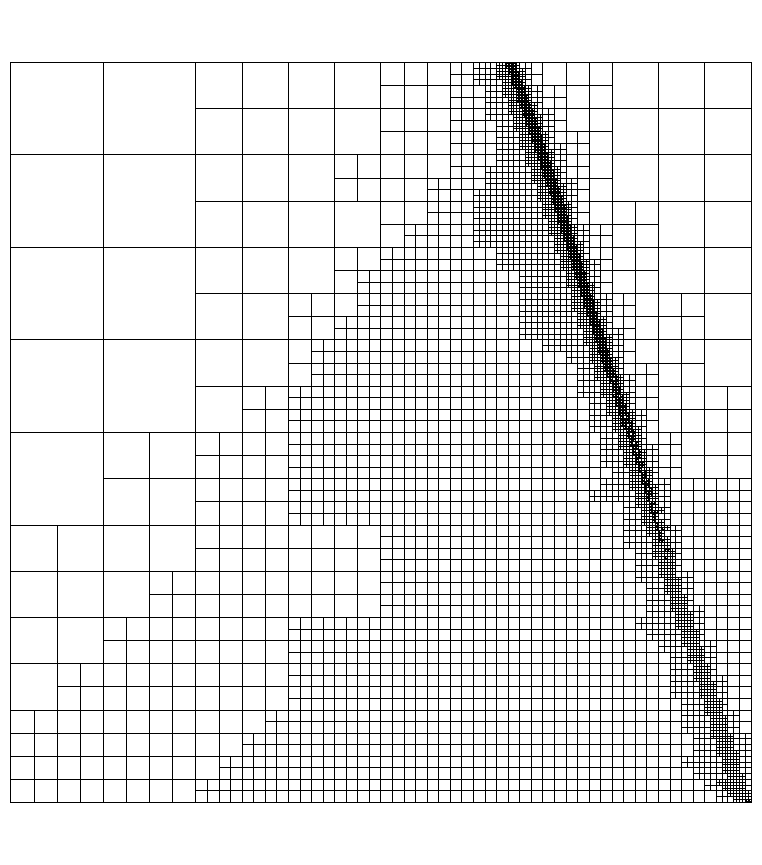
\includegraphics[width=\textwidth]{Dissertation/Noh/EntropyRobust-meshonly10.png}
% \caption{Final mesh with entropy scaled robust norm}
% \end{subfigure}
% \caption{Noh solution after 10 refinements}
% \label{fig:NohEntropyComparison}
% \end{figure}

% \begin{figure}[ht]
% \centering
% 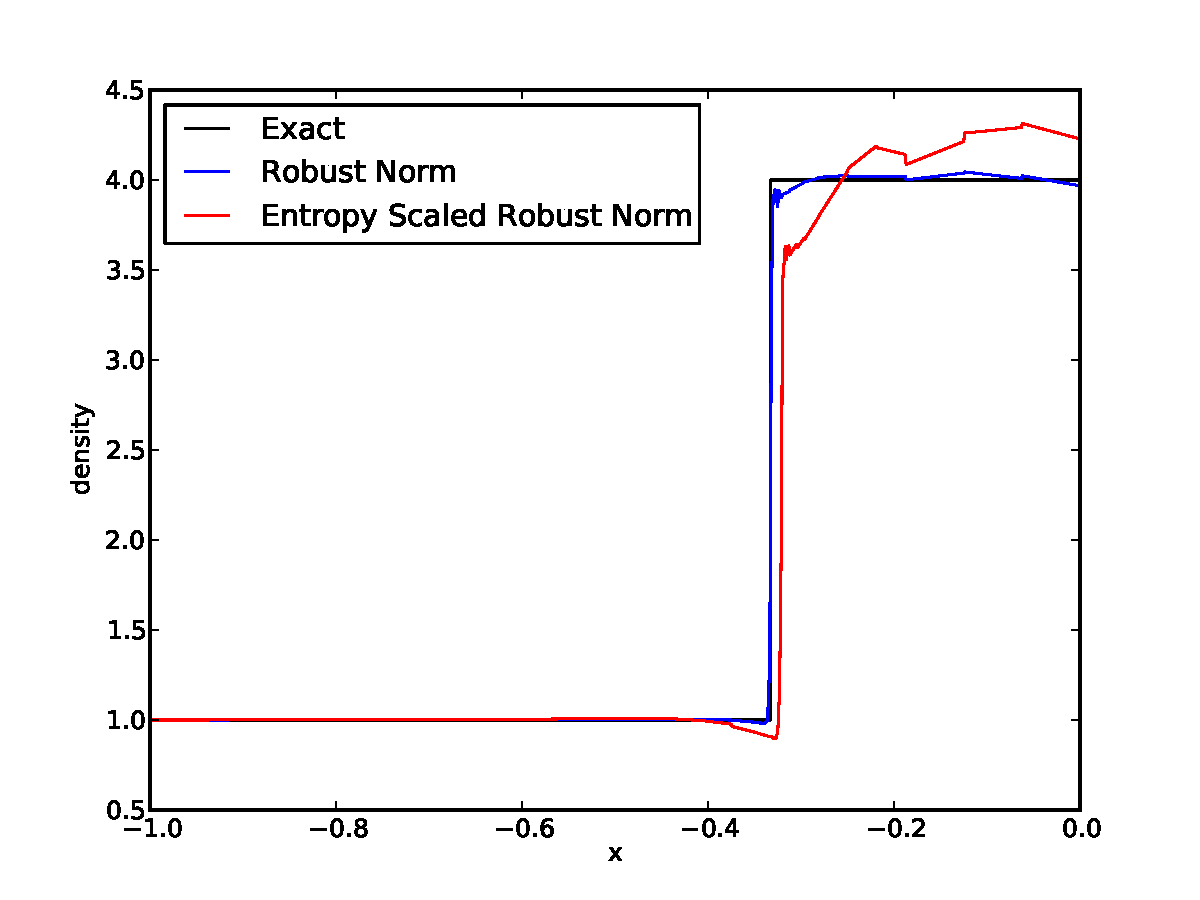
\includegraphics[width=0.9\textwidth]{Dissertation/Noh/EntropyNormComparison.pdf}
% \caption{Density at final time}
% \label{fig:NohEntropyComparison2}
% \end{figure}

\end{document}
